%-------------------
% About this template
%-------------------
% This template is based on the "Standard document" Overleaf template created by Christian L., which is distributed under the Creative Commons CC BY 4.0 license: https://cs.overleaf.com/latex/templates/standard-document/xhwhmfdcxhhj


%--------------------
% Packages
% -------------------
\documentclass[11pt,a4paper]{article}
\usepackage[utf8x]{inputenc}
\usepackage[T1]{fontenc}
%\usepackage{gentium}
% \usepackage{mathptmx} % Use Times Font

\usepackage[pdftex]{graphicx} % Required for including pictures
\usepackage[english]{babel} 
\usepackage[pdftex,linkcolor=black,pdfborder={0 0 0}]{hyperref} % Format links for pdf
\usepackage{calc} % To reset the counter in the document after title page
\usepackage{enumitem} % Includes lists
%\usepackage[utf8]{inputenc}%(only for the pdftex engine)


\frenchspacing % No double spacing between sentences
\linespread{1.2} % Set linespace
\usepackage[a4paper, lmargin=0.15\paperwidth, rmargin=0.15\paperwidth, tmargin=0.1\paperheight, bmargin=0.1\paperheight]{geometry} %margins
%\usepackage{parskip}

\usepackage[all]{nowidow} % Tries to remove widows
\usepackage[protrusion=true,expansion=true]{microtype} % Improves typography, load after fontpackage is selected

\graphicspath{ {./Figures} }

%-----------------------
% Set pdf information and add title, fill in the fields
%-----------------------
\hypersetup{ 	
pdfsubject = {ext4 file system overview},
pdftitle = {ext4 file system overview},
pdfauthor = {Phuriwat Angkoondittaphong}
}

%-----------------------
% Begin document
%-----------------------

%Please anonymize for submission
\begin{document} %

\title{ext4\footnote{In this report we use "ext4" instead of "Ext4", since many sources use it variously} file system overview}
\author{
{Phuriwat Angkoondittaphong}\\
{6388003 section 1}\\
{phuriwat.ang@student.mahidol.ac.th}
}
\date{}
\maketitle

\section{Introduction}

File system is essential part of the computer especially home computer that we use every day. Essentially, it is system that control persistence data structure inside the physical storage device such as disks, SSDs, magnetic tapes, etc. File system usually as 2 main goals, abstract user away from controlling the persistence data structure directly by using the API that file system provided and use resource as most efficient as possible in both time and space aspect. ~\cite{wiki:file_system}

ext4 was developed as extension of ext3, but due to stability reasons ext4 were born with partial backward compatible with ext3 and ext2. ext4 present itself as performance improved of ext3. ext4 has stable released on 21 October 2008 with Linux 2.6.28. Currently, ext4 is default file system of many Linux distributions such as Ubuntu and Debian. ~\cite{Ext4HowtoWiki, wiki:Ext4} 

\section{ext4 overview}
ext4 has the same architecture as ext2 and ext3 with change in parameters. Crop the disk into blocks and block groups. ~\cite{KernalDoc:Ext2}

\subsection{Block}
Each block can store some fixed size amount of data. It can be 1024, 2048, 4096 or 8192 bytes per block, depend on the system and configuration. ~\cite{KernalDoc:Ext2, opensource:intro_to_ext4fs}


\subsection{Block Group}
Each block group contain at maximum 8 blocks per group, first two preserved for block usage bitmap and inode usage bitmap, bitmap contain information which blocks and inodes are in use. When allocate the blocks, the algorithm tries to allocate all blocks in the same group first then allocate other group, in order to reduce the rotation and seek delay of the disk. ~\cite{KernalDoc:Ext2}

\subsection{Inode}
Inode represents a file in the system. It contains location of metadata and location of the block that it uses for store data. But if only a block is not enough, there is a pointer to an indirect block (which contains pointers to the next set of blocks), a pointer to a doubly-indirect block (which contains pointers to indirect blocks) and a pointer to a trebly-indirect block (which contains pointers to doubly-indirect blocks). ~\cite{KernalDoc:Ext2}

\subsection{Superblock}
There are blocks that store metadata of the file system, called superblock. It contains total number of inodes, blocks in the filesystem, the free one and etc. This information are important for porting the file system across machines. ~\cite{KernalDoc:Ext2} 


\subsection{Journal}
ext4 also inherited journal from ext3. ~\cite{wiki:Ext4} Journal is a file that responds for keep track of change in the file system before actually write back to the file system as checkpoint for data integrity. ~\cite{wiki:Journaling_file_system}

\begin{figure}[h]
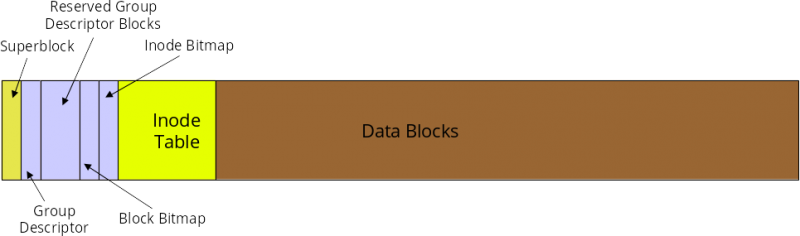
\includegraphics[width=\textwidth]{cylindergroup-01_1.png}
\caption{Block group structure.~\cite{opensource:intro_to_ext4fs}}
\end{figure}

\section{ext4 features}

\subsection{Block allocation by extents}
Instead of allocating indirect block (that we have mention in section 2) like in ext2, and ext3, which is not efficient for very big file, ext4 allows user to allocate contiguous of data block to reduce usage of pointer block, and reduction of fragmentation. ~\cite{opensource:intro_to_ext4fs}

\subsection{Multiblock allocation}

When ext2 and ext3 want to allocate the blocks, they allocate block one by one, which is inefficient. ext4 allows the file system to allocate multiple blocks per call using multiblock allocator (mballoc), instead of allocating one block per call, which eliminate overhead. ~\cite{Ext4HowtoWiki}

\subsection{Delayed allocation}

Traditionally (in ext3), the file system tried to allocate blocks as soon as possible even it wasn’t going to write immediately. But with delayed allocation in ext4, it waits while the file is kept in the cache, until it is really going to be written on the disk. ~\cite{Ext4HowtoWiki}

\subsection{Extended datetime range and precision}

ext4 uses higher precision datetime down to nanosecond resolution and extends datetime range to 1901 to 2446. ~\cite{wiki:Ext4, opensource:intro_to_ext4fs}

\subsection{Journal checksumming}

Recover file system from corrupted journal can lead to even more problems. So, ext4 checksum the journal to make sure it is not corrupted.~\cite{Ext4HowtoWiki}

\section{ext4 limitation}

ext4 has 1 EiB or $2^{60}$ of maximum file volume size, 16 TiB of maximum file size for 4 KiB block size and unlimited sub directories. ~\cite{Ext4HowtoWiki, wiki:Ext4}
Datetime uses in ext4 file system is limited to 14 Dec 1901 to 10 May 2446 only. ~\cite{wiki:Ext4}

\bibliographystyle{ieeetr}
\bibliography{bib}

\appendix

\end{document}
